% Options for packages loaded elsewhere
\PassOptionsToPackage{unicode}{hyperref}
\PassOptionsToPackage{hyphens}{url}
%
\documentclass[
]{article}
\usepackage{lmodern}
\usepackage{amssymb,amsmath}
\usepackage{ifxetex,ifluatex}
\ifnum 0\ifxetex 1\fi\ifluatex 1\fi=0 % if pdftex
  \usepackage[T1]{fontenc}
  \usepackage[utf8]{inputenc}
  \usepackage{textcomp} % provide euro and other symbols
\else % if luatex or xetex
  \usepackage{unicode-math}
  \defaultfontfeatures{Scale=MatchLowercase}
  \defaultfontfeatures[\rmfamily]{Ligatures=TeX,Scale=1}
\fi
% Use upquote if available, for straight quotes in verbatim environments
\IfFileExists{upquote.sty}{\usepackage{upquote}}{}
\IfFileExists{microtype.sty}{% use microtype if available
  \usepackage[]{microtype}
  \UseMicrotypeSet[protrusion]{basicmath} % disable protrusion for tt fonts
}{}
\makeatletter
\@ifundefined{KOMAClassName}{% if non-KOMA class
  \IfFileExists{parskip.sty}{%
    \usepackage{parskip}
  }{% else
    \setlength{\parindent}{0pt}
    \setlength{\parskip}{6pt plus 2pt minus 1pt}}
}{% if KOMA class
  \KOMAoptions{parskip=half}}
\makeatother
\usepackage{xcolor}
\IfFileExists{xurl.sty}{\usepackage{xurl}}{} % add URL line breaks if available
\IfFileExists{bookmark.sty}{\usepackage{bookmark}}{\usepackage{hyperref}}
\hypersetup{
  pdftitle={Kobe Bryant Shot Selection},
  pdfauthor={Laura Rodríguez Navas},
  hidelinks,
  pdfcreator={LaTeX via pandoc}}
\urlstyle{same} % disable monospaced font for URLs
\usepackage[margin=1in]{geometry}
\usepackage{color}
\usepackage{fancyvrb}
\newcommand{\VerbBar}{|}
\newcommand{\VERB}{\Verb[commandchars=\\\{\}]}
\DefineVerbatimEnvironment{Highlighting}{Verbatim}{commandchars=\\\{\}}
% Add ',fontsize=\small' for more characters per line
\usepackage{framed}
\definecolor{shadecolor}{RGB}{248,248,248}
\newenvironment{Shaded}{\begin{snugshade}}{\end{snugshade}}
\newcommand{\AlertTok}[1]{\textcolor[rgb]{0.94,0.16,0.16}{#1}}
\newcommand{\AnnotationTok}[1]{\textcolor[rgb]{0.56,0.35,0.01}{\textbf{\textit{#1}}}}
\newcommand{\AttributeTok}[1]{\textcolor[rgb]{0.77,0.63,0.00}{#1}}
\newcommand{\BaseNTok}[1]{\textcolor[rgb]{0.00,0.00,0.81}{#1}}
\newcommand{\BuiltInTok}[1]{#1}
\newcommand{\CharTok}[1]{\textcolor[rgb]{0.31,0.60,0.02}{#1}}
\newcommand{\CommentTok}[1]{\textcolor[rgb]{0.56,0.35,0.01}{\textit{#1}}}
\newcommand{\CommentVarTok}[1]{\textcolor[rgb]{0.56,0.35,0.01}{\textbf{\textit{#1}}}}
\newcommand{\ConstantTok}[1]{\textcolor[rgb]{0.00,0.00,0.00}{#1}}
\newcommand{\ControlFlowTok}[1]{\textcolor[rgb]{0.13,0.29,0.53}{\textbf{#1}}}
\newcommand{\DataTypeTok}[1]{\textcolor[rgb]{0.13,0.29,0.53}{#1}}
\newcommand{\DecValTok}[1]{\textcolor[rgb]{0.00,0.00,0.81}{#1}}
\newcommand{\DocumentationTok}[1]{\textcolor[rgb]{0.56,0.35,0.01}{\textbf{\textit{#1}}}}
\newcommand{\ErrorTok}[1]{\textcolor[rgb]{0.64,0.00,0.00}{\textbf{#1}}}
\newcommand{\ExtensionTok}[1]{#1}
\newcommand{\FloatTok}[1]{\textcolor[rgb]{0.00,0.00,0.81}{#1}}
\newcommand{\FunctionTok}[1]{\textcolor[rgb]{0.00,0.00,0.00}{#1}}
\newcommand{\ImportTok}[1]{#1}
\newcommand{\InformationTok}[1]{\textcolor[rgb]{0.56,0.35,0.01}{\textbf{\textit{#1}}}}
\newcommand{\KeywordTok}[1]{\textcolor[rgb]{0.13,0.29,0.53}{\textbf{#1}}}
\newcommand{\NormalTok}[1]{#1}
\newcommand{\OperatorTok}[1]{\textcolor[rgb]{0.81,0.36,0.00}{\textbf{#1}}}
\newcommand{\OtherTok}[1]{\textcolor[rgb]{0.56,0.35,0.01}{#1}}
\newcommand{\PreprocessorTok}[1]{\textcolor[rgb]{0.56,0.35,0.01}{\textit{#1}}}
\newcommand{\RegionMarkerTok}[1]{#1}
\newcommand{\SpecialCharTok}[1]{\textcolor[rgb]{0.00,0.00,0.00}{#1}}
\newcommand{\SpecialStringTok}[1]{\textcolor[rgb]{0.31,0.60,0.02}{#1}}
\newcommand{\StringTok}[1]{\textcolor[rgb]{0.31,0.60,0.02}{#1}}
\newcommand{\VariableTok}[1]{\textcolor[rgb]{0.00,0.00,0.00}{#1}}
\newcommand{\VerbatimStringTok}[1]{\textcolor[rgb]{0.31,0.60,0.02}{#1}}
\newcommand{\WarningTok}[1]{\textcolor[rgb]{0.56,0.35,0.01}{\textbf{\textit{#1}}}}
\usepackage{graphicx,grffile}
\makeatletter
\def\maxwidth{\ifdim\Gin@nat@width>\linewidth\linewidth\else\Gin@nat@width\fi}
\def\maxheight{\ifdim\Gin@nat@height>\textheight\textheight\else\Gin@nat@height\fi}
\makeatother
% Scale images if necessary, so that they will not overflow the page
% margins by default, and it is still possible to overwrite the defaults
% using explicit options in \includegraphics[width, height, ...]{}
\setkeys{Gin}{width=\maxwidth,height=\maxheight,keepaspectratio}
% Set default figure placement to htbp
\makeatletter
\def\fps@figure{htbp}
\makeatother
\setlength{\emergencystretch}{3em} % prevent overfull lines
\providecommand{\tightlist}{%
  \setlength{\itemsep}{0pt}\setlength{\parskip}{0pt}}
\setcounter{secnumdepth}{-\maxdimen} % remove section numbering

\title{\textbf{Kobe Bryant Shot Selection}}
\author{Laura Rodríguez Navas}
\date{2020-05-22}

\begin{document}
\maketitle

\hypertarget{introducciuxf3n}{%
\section{\texorpdfstring{\textbf{Introducción}}{Introducción}}\label{introducciuxf3n}}

Este proyecto lleva a cabo un proyecto completo de Ciencia de Datos
donde vamos a analizar, transformar, modelar y evaluar un conjunto de
datos de Kaggle (\url{https://www.kaggle.com/}). Concretamente, para
este proyecto se ha usado un conjunto de datos que describe los aciertos
y fallos de lanzamientos a canasta del jugador de baloncesto Kobe Bryant
durante 20 años de su carrera en la NBA
(\url{https://www.kaggle.com/c/kobe-bryant-shot-selection/data}).

La tarea del proyecto es predecir si los lanzamientos a canastas de Kobe
Bryant entraron o no en el aro (``shot\_made\_flag''), es decir, los
lanzamientos acertados. Del conjunto de datos se han eliminado 5000
valores de este atributo (representados como valores faltantes en el
conjunto de datos). Estos datos serán el conjunto de prueba sobre el
cual se realizará la predicción.

El conjunto de datos contiene 30697 (25697 + 5000) instancias y un gran
número de variables explicativas (11 discretas y 14 numéricas). Estas 25
variables (incluyendo la clase a predecir shot\_made\_flag) se centran
en la descripción cualitativa y cuantitativa de multitud de aspectos de
cada uno de los lanzamientos de Kobe Bryant.

\begin{verbatim}
## 'data.frame':    30697 obs. of  25 variables:
##  $ action_type       : Factor w/ 57 levels "Alley Oop Dunk Shot",..: 27 27 27 27 6 27 28 27 27 42 ...
##  $ combined_shot_type: Factor w/ 6 levels "Bank Shot","Dunk",..: 4 4 4 4 2 4 5 4 4 4 ...
##  $ game_event_id     : int  10 12 35 43 155 244 251 254 265 294 ...
##  $ game_id           : int  20000012 20000012 20000012 20000012 20000012 20000012 20000012 20000012 20000012 20000012 ...
##  $ lat               : num  34 34 33.9 33.9 34 ...
##  $ loc_x             : int  167 -157 -101 138 0 -145 0 1 -65 -33 ...
##  $ loc_y             : int  72 0 135 175 0 -11 0 28 108 125 ...
##  $ lon               : num  -118 -118 -118 -118 -118 ...
##  $ minutes_remaining : int  10 10 7 6 6 9 8 8 6 3 ...
##  $ period            : int  1 1 1 1 2 3 3 3 3 3 ...
##  $ playoffs          : int  0 0 0 0 0 0 0 0 0 0 ...
##  $ season            : Factor w/ 20 levels "1996-97","1997-98",..: 5 5 5 5 5 5 5 5 5 5 ...
##  $ seconds_remaining : int  27 22 45 52 19 32 52 5 12 36 ...
##  $ shot_distance     : int  18 15 16 22 0 14 0 2 12 12 ...
##  $ shot_made_flag    : int  NA 0 1 0 1 0 1 NA 1 0 ...
##  $ shot_type         : Factor w/ 2 levels "2PT Field Goal",..: 1 1 1 1 1 1 1 1 1 1 ...
##  $ shot_zone_area    : Factor w/ 6 levels "Back Court(BC)",..: 6 4 3 5 2 4 2 2 4 2 ...
##  $ shot_zone_basic   : Factor w/ 7 levels "Above the Break 3",..: 5 5 5 5 6 5 6 6 3 3 ...
##  $ shot_zone_range   : Factor w/ 5 levels "16-24 ft.","24+ ft.",..: 1 3 1 1 5 3 5 5 3 3 ...
##  $ team_id           : int  1610612747 1610612747 1610612747 1610612747 1610612747 1610612747 1610612747 1610612747 1610612747 1610612747 ...
##  $ team_name         : Factor w/ 1 level "Los Angeles Lakers": 1 1 1 1 1 1 1 1 1 1 ...
##  $ game_date         : Factor w/ 1559 levels "1996-11-03","1996-11-05",..: 311 311 311 311 311 311 311 311 311 311 ...
##  $ matchup           : Factor w/ 74 levels "LAL @ ATL","LAL @ BKN",..: 29 29 29 29 29 29 29 29 29 29 ...
##  $ opponent          : Factor w/ 33 levels "ATL","BKN","BOS",..: 26 26 26 26 26 26 26 26 26 26 ...
##  $ shot_id           : int  1 2 3 4 5 6 7 8 9 10 ...
\end{verbatim}

\hypertarget{exploraciuxf3n-de-datos}{%
\section{\texorpdfstring{\textbf{Exploración de
datos}}{Exploración de datos}}\label{exploraciuxf3n-de-datos}}

Al principio podemos ver que la variable clase a predecir (atributo
\emph{``shot\_made\_flag''}) se distribuye de manera bastante
equitativa. No realizaremos ninguna acción para tratar con el conjunto
de datos desequilibrado.

\begin{center}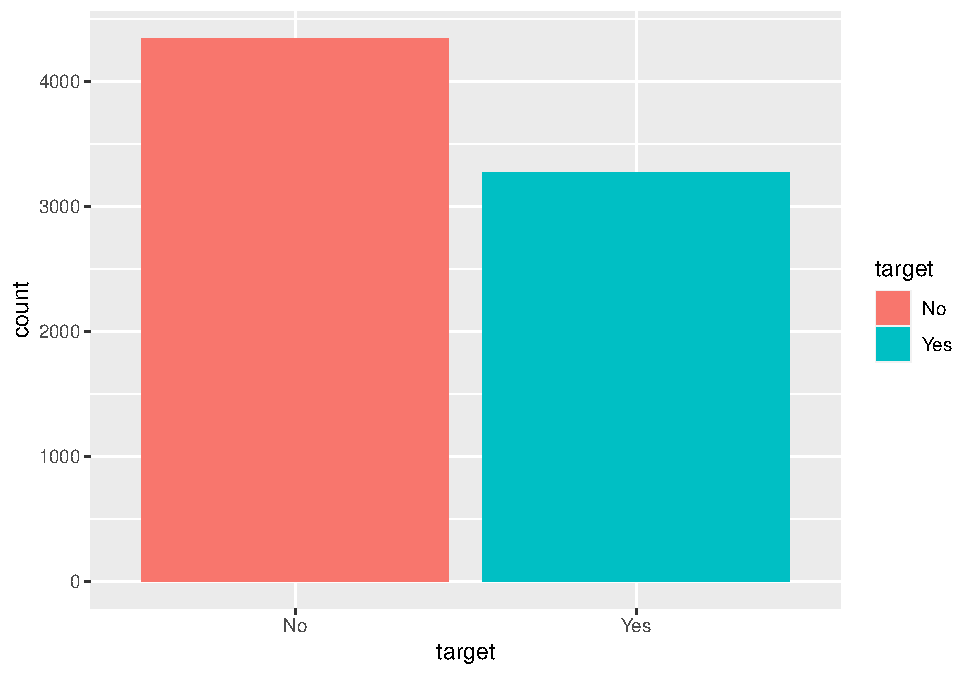
\includegraphics{document_files/figure-latex/unnamed-chunk-4-1} \end{center}

Precisión de los lanzamientos por temporada (atributo
\emph{``season''}).

\begin{center}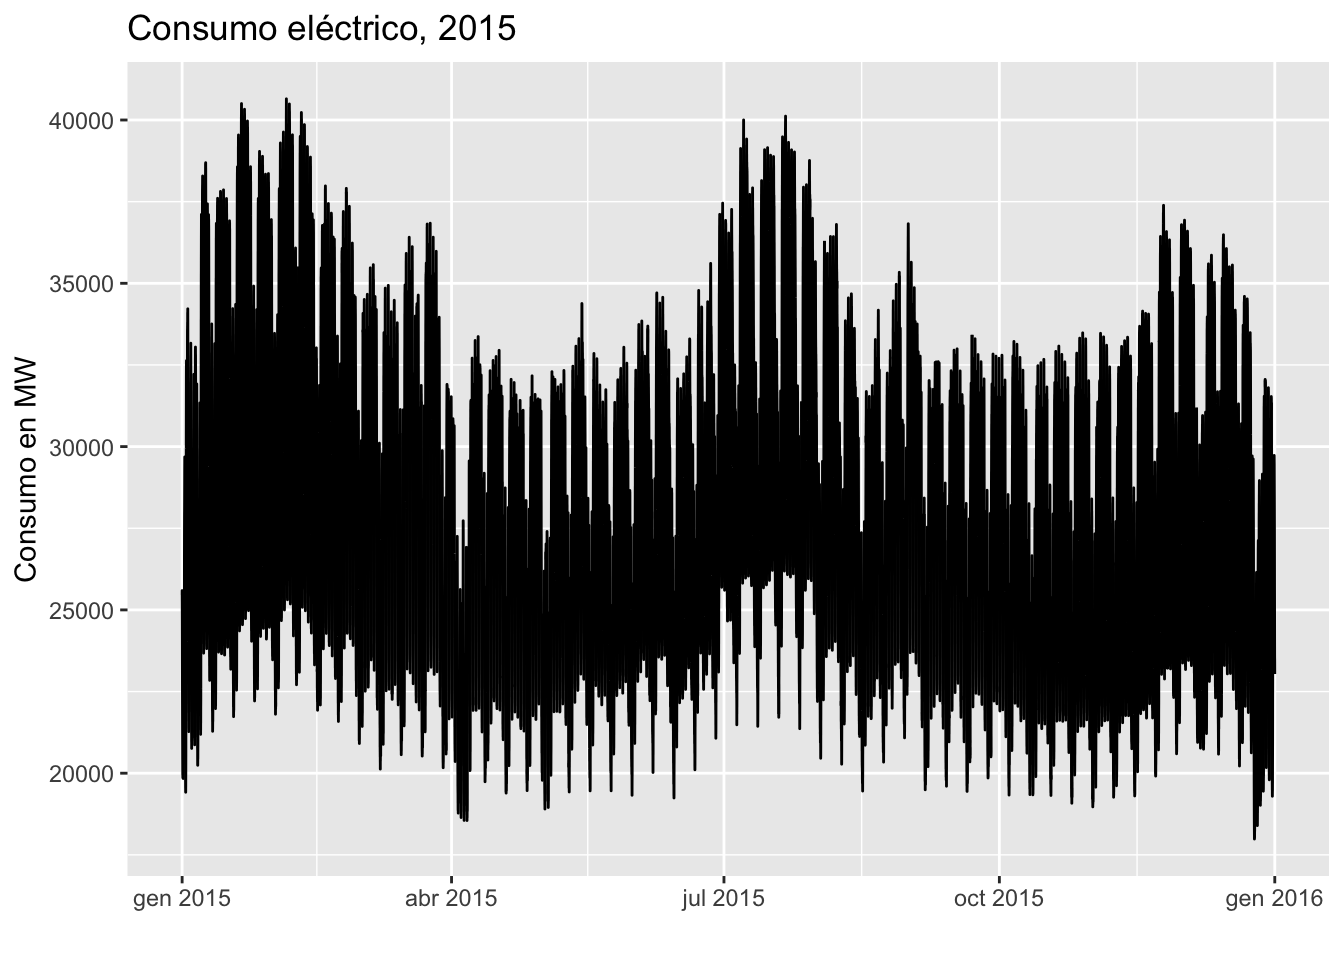
\includegraphics{document_files/figure-latex/unnamed-chunk-5-1} \end{center}

Precisión de los lanzamientos por temporada (atributo
\emph{``shot\_distance''}).

\begin{center}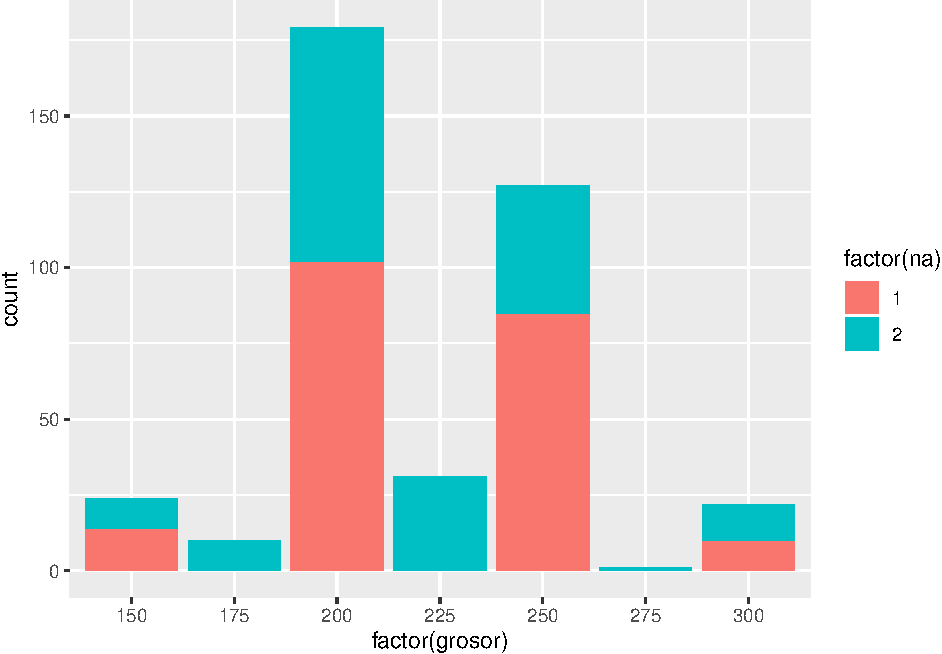
\includegraphics{document_files/figure-latex/unnamed-chunk-6-1} \end{center}

\hypertarget{selecciuxf3n-de-variables}{%
\subsection{\texorpdfstring{\textbf{Selección de
variables}}{Selección de variables}}\label{selecciuxf3n-de-variables}}

Reduzimos la cantidad de variables para un análisis más fácil dividiendo
el conjunto de datos en un conjunto de datos de entrenamiento y un
conjunto de datos de evaluación (test).

\begin{Shaded}
\begin{Highlighting}[]
\NormalTok{train <-}\StringTok{ }\NormalTok{data[}\OperatorTok{!}\KeywordTok{is.na}\NormalTok{(data}\OperatorTok{$}\NormalTok{shot_made_flag), ]}
\KeywordTok{any}\NormalTok{(}\KeywordTok{is.na}\NormalTok{(train))}
\end{Highlighting}
\end{Shaded}

\begin{verbatim}
## [1] FALSE
\end{verbatim}

\begin{Shaded}
\begin{Highlighting}[]
\NormalTok{test <-}\StringTok{ }\NormalTok{data[}\KeywordTok{is.na}\NormalTok{(data}\OperatorTok{$}\NormalTok{shot_made_flag), ]}
\KeywordTok{any}\NormalTok{(}\KeywordTok{is.na}\NormalTok{(test))}
\end{Highlighting}
\end{Shaded}

\begin{verbatim}
## [1] TRUE
\end{verbatim}

\hypertarget{limpieza-de-datos}{%
\subsection{\texorpdfstring{\textbf{Limpieza de
datos}}{Limpieza de datos}}\label{limpieza-de-datos}}

Asumimos la independencia de cada lanzamiento, por lo tanto, las
siguientes columnas pueden descartarse.

\begin{itemize}
\tightlist
\item
  \textbf{game\_event\_id}. Indepeniente al análisis.
\item
  \textbf{game\_id}. Indepeniente al análisis.
\item
  \textbf{loc\_x}
\item
  \textbf{loc\_y}
\item
  \textbf{lat}. Correlacionada con loc\_x.
\item
  \textbf{lon}. Correlacionada con loc\_y.
\item
  \textbf{shot\_zone\_area}
\item
  \textbf{shot\_zone\_basic}
\item
  \textbf{shot\_zone\_range}
\item
  \textbf{team\_id}. Siempre es el mismo número.
\item
  \textbf{team\_name}. Siempre es el mismo valor: \emph{LA Lakers}.
\item
  \textbf{game\_date}
\item
  \textbf{matchup}
\end{itemize}

\hypertarget{transformaciuxf3n-de-datos}{%
\subsection{\texorpdfstring{\textbf{Transformación de
datos}}{Transformación de datos}}\label{transformaciuxf3n-de-datos}}

Las columnas \emph{``minutes\_remaining''} y
\emph{``seconds\_remaining''} pueden descartarse.

\hypertarget{modelado}{%
\section{\texorpdfstring{\textbf{Modelado}}{Modelado}}\label{modelado}}

Una vez se ha realizado el análisis sobre los datos, incluyendo la
limpieza, transformación y generación de nuevas variables interesantes
para el estudio, pasamos a la fase del modelado.

\hypertarget{evaluaciuxf3n}{%
\section{\texorpdfstring{\textbf{Evaluación}}{Evaluación}}\label{evaluaciuxf3n}}

\hypertarget{conclusiones}{%
\section{\texorpdfstring{\textbf{Conclusiones}}{Conclusiones}}\label{conclusiones}}

\hypertarget{resultado-de-kaggle}{%
\section{\texorpdfstring{\textbf{Resultado de
Kaggle}}{Resultado de Kaggle}}\label{resultado-de-kaggle}}

\end{document}
